\section{The ORCHID-SAGE standard}
\label{sec:methods}

Regenerating a CALPHAD assessment requires two distinct elements: a method describing how experimental and computational evidence is transformed into model parameters and a record of applying that method to a particular system. In ORCHID-SAGE, the method is specified in a general protocol, while the record consists of a small set of structured documents that conform to a common schema. Because all operations--- from selecting evidence and building the one-shot PhaseForge model to optimizing parameters and quantifying their uncertainty---must be documented using this schema, the schema largely determines which parts of an assessment can be reproduced. The description of the standard therefore begins with the documents and their schema.

\subsection{Protocol levels and the schema}
\label{sec:methods:levels}

An assessment consists of a sequence of three kinds of operations (deterministic calculations, numerical optimizations, and decisions requiring judgment), and regenerating its result requires a record of all three. ORCHID-SAGE maintains this record at three levels. The general protocol, at the \textbf{first level}, describes the method in a form applicable to any (binary) system. This protocol is versioned, so that the version used in this work (\texttt{orchid-calphad-fit}, version 2.1.2) can be cited unambiguously, and its written rationale is fixed through a SHA-256 hash. The specific protocol, at the \textbf{second level}, instantiates the general protocol for a single database and is linked to it through an identifier, version, and file hash. It contains the hashed inputs, the departures from the general protocol, the selected evidence, all executed runs (including failed ones), and the decisions taken, together with the person or algorithm responsible for each decision and the corresponding justification. Run cards, at the \textbf{third level}, document individual executions, including the host, interpreter, and installed packages; the exact command; the random seeds; the hashed inputs and outputs; and the optimizer trajectory. The specific protocol thus constitutes the assessment plan, while the run cards record its execution (\cref{fig:standard}).

\begin{figure}[tbp]
    \centering
    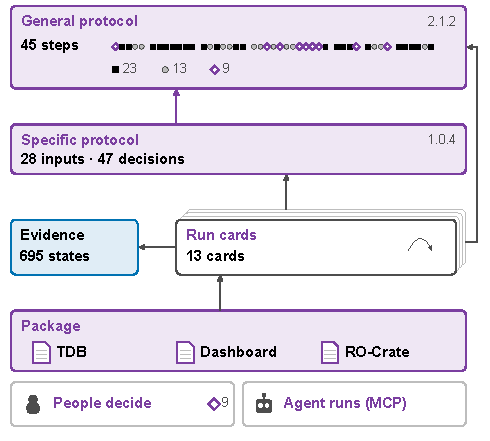
\includegraphics[width=83mm]{fig_crni_standard_1col}
    \caption{The ORCHID-SAGE standard, shown for Cr--Ni. The general protocol describes the method in steps of three kinds (deterministic, numerical and judgment), the specific protocol applies it to one database with its inputs, runs and decisions, and the run cards record each execution. The package delivers the database with its header, the dashboard, and the record as an RO-Crate, in which the arrows correspond to PROV relations. People decide at the judgment steps, and an agent can run the specific protocol through the ORCHID-SAGE server.}
    \label{fig:standard}
\end{figure}

Because the same documents are supposed to be read by humans and machines, the three levels are defined within a single schema family, \texttt{orchid-assessment-schema} (version 1.0.0-draft.2 at the time of writing), written in JSON Schema and applied to documents in a restricted subset of YAML. The organization of a protocol follows the HowTo vocabulary of schema.org~\cite{schemaorg_howto}, which divides a procedure into sections and steps. Each step includes an imperative description sufficient for execution, the supplies and tools it requires, and the results it produces. However, this vocabulary does not distinguish between steps with an outcome fully determined by their inputs and steps that depend on numerical approximations or human judgment. For this reason, the schema introduces the kind of each step, which specifies the outcome expected from a rerun: byte-identical outputs for deterministic steps, agreement within declared tolerances for numerical steps and, for judgment steps, the explicit statement of the decision rule and of the person responsible for the decision. A validator finally verifies the complete record, confirming that the documents conform to the schema, that the referenced files exist with the recorded hashes, and that no step consumes an input before it has been produced.

The checks attached to the steps of a protocol serve two different purposes.~\textbf{Gates} check process integrity and record completeness. They verify, for example, that the fitting software matches the declared build, that the pure-element limits are reproduced, that excluded phases are specified at each observed state, that inputs and outputs match their recorded hashes, and that the optimizer's trajectory is stored. Before releasing a database, an independent rerun on a different machine must also agree with the original assessment. An assessment that fails any gate is considered incomplete, regardless of how well it fits the data (\cref{fig:gates}). In contrast, \textbf{fit quality} is not judged by a pass-or-fail criterion applied to a single figure of merit. Instead, we rank candidate fits first by the plausibility of the model's energy scale, then by the topology of the calculated phase diagram, and finally by quantitative agreement with the (ORCHID) data. We then select the most reasonable fit (\cref{sec:methods:sequence}). 

\begin{figure}[tbp]
    \centering
    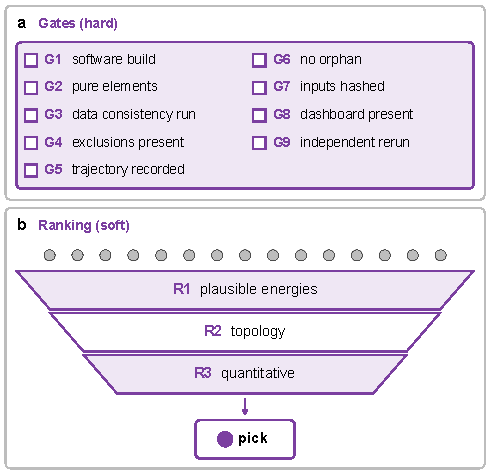
\includegraphics[width=83mm]{fig_gates_ranking_1col}
    \caption{Gates and ranking in the general protocol. (a)~The nine gates check the integrity of the process and of the record, and an assessment that fails any of them is incomplete, however well it fits the data. (b)~Candidate fits are not gated but ranked, first by the plausibility of their energies, then by topology and finally by quantitative agreement, and the most reasonable fit is picked with its misses reported as notes. Both panels are schematic.}
    \label{fig:gates}
\end{figure}

The ranking assesses the quality of the fit, while the tolerances of the numerical steps determine whether a fit has been reproduced. Here, we note that these tolerances must account for the fact that the fitness landscape of the CALPHAD model is often nearly flat in some regions of the parameter space, and, in these directions, a rerun can cause large changes in individual parameters with minimal changes to Gibbs energies and thermodynamic observables. Thus, it is more meaningful to compare the databases' predictions than their parameters. When a rerun produces similar observables under identical protocols it is then asserted that the protocol is \emph{reproducible}.

\subsection{Evidence from ORCHID}
\label{sec:methods:orchid}

\begin{figure}[tbp]
    \centering
    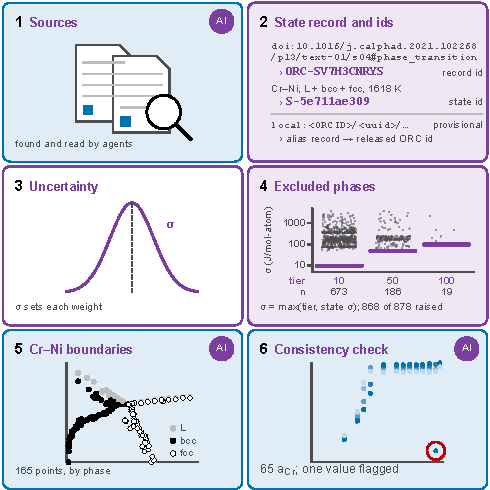
\includegraphics[width=83mm]{fig_orchid_evidence}
    \caption{Evidence used in this work. (1)~Sources are found and read by AI agents. (2)~Each value is stored as a record of a fully defined state, with a record id derived from its source (here the Cr--Ni eutectic, ORC-SV7H3CNRYS) and a state id derived from the state itself. (3)~The uncertainty of each record sets its weight in the fit. (4)~Excluded phases enter with an energy scale set by their certainty tier or by the uncertainty of the state, whichever is larger. (5)~The 165 Cr--Ni phase-boundary points. (6)~The consistency check on the activities of Pugliese and Fitterer~\cite{pugliese1970}, with one inconsistent value flagged, not changed. ORCHID v2026.10 and records extracted for this work; record identifiers are provided with the source data.}
    \label{fig:orchid}
\end{figure}

Among the inputs to a CALPHAD assessment, the experimental evidence is the most difficult to trace and extract (it is dispersed in non-machine-readable forms), and for this reason, it is the first element to be fixed in the record. The evidence here comes from ORCHID~\cite{arroyave2026orchid}, which stores each (AI-extracted) value reported in the literature as an observation of a fully defined equilibrium state (\cref{fig:orchid}). For Cr--Ni (used in this work as an example), ORCHID's public release contains 42 accepted values, mostly corresponding to invariant reactions, phase transitions, and calculated enthalpies, but no experimental thermochemical data for the liquid and solid solutions. Therefore, AI agents were used to follow the citation chains of the existing assessments, retrieve the articles that were not available locally, and extract, using the ORCHID schema, the data compiled by Hao et al.~\cite{hao2021} as well as the Cr activities measured by Pugliese and Fitterer~\cite{pugliese1970}. In each case, the value was traced to the publication in which it was first reported.

For use in a reproducible assessment, these observations must be independently identifiable. ORCHID records carry identifiers derived from the locator of the value in the source (for example, the DOI of the paper together with the table and row in which the value appears). The equilibrium states observed in these records receive unique identifiers of their own, obtained as a hash of a canonical description of the state that includes the system, the phases, the pressure and the coordinates, so that \emph{two people describing the same state arrive at the same identifier}. Data not yet released by ORCHID, such as the new extractions of this work, are assigned identifiers in a provisional namespace constructed from the ORCID of the contributor and an identifier of the dataset. Upon publication, these provisional identifiers are linked to the released ones through alias records, and they are never rewritten or reused. Each state in the evidence of an assessment thus carries either its ORCHID identifiers and the release in which they appear, or the reason why this link is still missing, together with a reference to the intake through which it will be resolved.

When performing a CALPHAD model fit, different pieces of evidence must be provided with a statistical weight~\cite{bocklund2019espei} that is in turn used to compute to the likelihood (or model error) of the CALPHAD fit. Rather than assigning these uncertainties 'by hand', we take this uncertainty from the source when reported there. Otherwise, we use the calibration of the corresponding measurement method in ORCHID. 

We note that an 'observation' contains more information than what has been directly observed or inferred, e.g., the location of a phase boundary, the phases present at a given composition and temperature, a thermo-chemical measurement. In fact, what has \emph{not been observed} is also valid (and, in some cases even stronger) evidence. More specifically, if an expert human assessor is fairly certain of the phases likely to be present in the equilibrium state under given thermodynamic conditions, then they can also be certain of the phases that \textbf{must not be} part of that state. 

For this reason, the ORCHID standard requires the definition of a list of excluded phases at all observed states, including single-phase states, and a dataset without this list is considered incomplete, although the absence of a so-excluded phase is never claimed to be proven. The strength of an exclusion depends on the \emph{thermodynamic distance} between the state and the excluded phase field, measured relative to the state's uncertainty in temperature and composition, and is expressed through certainty tiers that set the energy scale of the corresponding term in the objective function. This energy scale can be understood to be a minimal distance away from the equilibrium hyper-plane (or convex hull) at a given thermodynamic condition. A scale of \qty{10}{\J\per\mole} of atoms is assigned when the state lies more than three uncertainties away from any observed field or boundary of the phase and no source reports the phase there, a scale of \qty{50}{\J\per\mole} when the state lies closer or the exclusion rests on a single source, and a scale of \qty{100}{\J\per\mole} when the state is adjacent to the boundary of the phase or the exclusion is assumed from a diagram or contested. 

This three-tiered scale reflects the degree of 'thermodynamic certainty' that can be assigned to a phase exclusion, with higher tiers corresponding to larger uncertainty. The assigned tier, however, sets only a lower bound, since the scale used is the larger of the tier and the state's uncertainty, converted to energy through the entropy change across the boundary. In this way, an exclusion can never be held more tightly than the measurement on which it rests allows, and it is the evidence, not the default settings of the fitting software (ESPEI in this case~\cite{bocklund2019espei}), that determines how strongly the phase diagram's topology is held in place.

Before entering the fit, the data are also checked for internal consistency. For Cr--Ni, the AI agents carried out this check and found that the activity of 0.112 printed by Pugliese and Fitterer~\cite{pugliese1970} at 95~at.\% Cr and \qty{1448}{\K} cannot be reconciled with the cell potential reported in the same row of their table, which is almost identical to those of the neighboring alloys. The same agents also found that one of the phase-boundary datasets contains six repeated rows. We note that neither finding changes the data, since the suspect activity is kept with a flag and enters the fit with its uncertainty, while the repeated rows are counted only once.

Once checked, the evidence read by the fit is frozen in a versioned evidence bundle. This bundle contains the datasets and the files of excluded phases exactly as they are read by the objective function, the observations derived from the one-shot model constructed using PhaseForge~\cite{zhu2025accelerating} and the inputs required for a rerun, together with a record of the observed states, their certainty tiers and their links to ORCHID. A manifest lists the SHA-256 hash of each of these files as well as a hash of the bundle as a whole. Since a bundle is never overwritten, any change in the evidence, including correcting an error, produces a new version of the bundle, which can then be cited by a new version of the specific protocol. Only derived facts enter the bundle, whereas restricted sources are referred to only through their hashes and are not redistributed. A rerun thus requires only the bundle, while the original sources are needed only to rebuild the bundle from the beginning.

\subsection{The one-shot model}
\label{sec:methods:phaseforge}

After specifying the evidence, the next element of the record is the model used as the starting point for the fit. In this work, this starting point is the one-shot model obtained using PhaseForge~\cite{zhu2025accelerating,zhu2025machinelearningpotentialsalloys}, constructed entirely from energetics calculated with a MLIP. The model construction procedure is part of the general protocol, so it cannot be changed between assessments without a recorded decision. In the one-shot model, the Gibbs energies of the end-members are taken from the SGTE descriptions of the pure elements~\cite{dinsdale1991sgte}, while the potential is used to calculate the mixing energy of each phase relative to the pure elements on the same lattice. This makes the model compatible with existing thermodynamic databases.

For the bcc and fcc solid solutions, we obtained the mixing energies from 128-atom special quasirandom structures (SQS)~\cite{zunger1990special}, generated with m\_scraps~\cite{arroyave2026mscraps,singh2021scraps} using two different seeds at each composition, so the spread between the two seeds provides an estimate of the configurational uncertainty. We evaluated these structures with the GRACE-2L-SMAX-OMAT-large potential~\cite{bochkarev2024grace}, using GRACE-2L-OMAT as a cross-check. A random arrangement of atoms on a lattice that is intrinsically unstable at a given composition tends to transform during relaxation, and the energy obtained this way no longer corresponds to the phase being modeled. To detect such transformations, we relaxed each structure in stages: first in volume, then in volume and ionic positions, and finally in cell shape, and checked the lattice after each stage. The energy after the relaxation of volume and ions is the value used in the model, while the interval between the unrelaxed and the fully relaxed energies defines its uncertainty. In Cr--Ni, the bcc structures with $x_{\mathrm{Ni}} \geq 0.5$ and the fcc structures with $x_{\mathrm{Ni}} \leq 0.31$ transformed even at this intermediate stage. Instead of being discarded, these structures enter the model with the midpoint of the interval as their value and half of the interval as their uncertainty, reflecting the fact that their energy is only known to lie between these two limits (\cref{fig:energetics}a).


\begin{figure}[tbp]
    \centering
    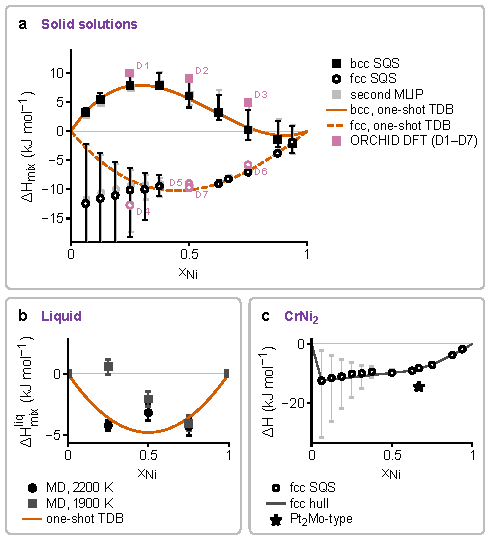
\includegraphics[width=83mm]{fig_crni_energetics_1col}
    \caption{Energetics of the one-shot model of Cr--Ni, in \unit{\kilo\joule\per\mole} of atoms. (a)~Mixing enthalpies of the bcc (squares) and fcc (circles) SQS, calculated with GRACE-2L-SMAX-OMAT-large (black) and GRACE-2L-OMAT (grey), with the interval between the unrelaxed and fully relaxed energies as error bars, the Redlich--Kister terms of the one-shot model (orange) and the DFT records of ORCHID (pink)~\cite{liu2016alcocrni,bracq2021enthalpy}. (b)~Mixing enthalpy of the liquid from molecular dynamics at \qty{2200}{\K} and \qty{1900}{\K}, with the single term of the one-shot model. (c)~CrNi$_2$ against the fcc SQS and their convex hull. ORCHID v2026.10; record identifiers are provided with the source data.}
    \label{fig:energetics}
\end{figure}

The mixing energies were then fitted with Redlich--Kister polynomials, with the interaction parameters defined in alphabetical order of the elements, as is the convention in CALPHAD databases. Since there is no evidence of chemical ordering in the fcc or bcc solid solutions of this system, these phases are described as disordered solutions (\texttt{FCC\_A1}, or \texttt{BCC\_A2} in Strukturbericht designation ), while CrNi$_2$, which has the Pt$_2$Mo structure, is described as a stoichiometric compound with a formation energy calculated with the same potential (\cref{fig:energetics}c). 

When the one-shot model is later refined against experimental data, its mixing and formation energies enter the fit as observations in their own right, so the refined model cannot depart from them without a cost. Each observation is assigned an uncertainty of \qty{9.7}{\kilo\joule\per\mole} of atoms, corresponding to the typical difference between energies calculated with the density functional theory on which the potential is trained and calorimetric measurements~\cite{kirklin2015oqmd,arroyave2026orchid}.

Unlike the solid phases, the liquid cannot be represented by static structures, so we calculated its mixing energy through molecular dynamics simulations with the same potential. We performed simulations with 108 atoms in five compositions, including pure liquids as references, and at two temperatures: \qty{2200}{\K}, just above the melting point of Cr, and \qty{1900}{\K}. In all cases, production runs of \qty{100}{\ps} followed the melting and equilibration of the cell, and the liquid character of the final configuration was confirmed through the mean-square displacement of the atoms. We assessed the effect of cell size with an additional simulation of 864 atoms at $x_{\mathrm{Ni}} = 0.5$ and \qty{2200}{\K} (\cref{sec:methods:entropy}). The enthalpy of mixing at each temperature corresponds to the average total energy, including the $pV$ term, relative to that of the pure liquids (\cref{fig:energetics}b), and these enthalpies were fitted with a single Redlich--Kister parameter, the temperature dependence of which is determined by the excess entropy of the liquid (\cref{sec:methods:entropy}). This description of the liquid, together with the solid-phase energies, completes the one-shot database. The database and the phase diagram calculated with it in pycalphad~\cite{otis2017pycalphad} thus constitute the first result of the assessment, and the reference against which the subsequent refinement is measured.

\subsection{Liquid entropy}
\label{sec:methods:entropy}

Because the mixing enthalpies at two temperatures are insufficient to determine the temperature dependence of the liquid parameters, we also estimated the excess entropy of the liquid from molecular dynamics simulations, following the method proposed by Hong and Liu~\cite{hong2025entropy}. In this method, the entropy of the liquid is separated into two contributions, a vibrational one, obtained from the spectrum of the velocity autocorrelation function, and a configurational one, accounting for the chemical mixing of the two species. In its original form, however, the chemical-mixing term does not reduce to the ideal entropy of mixing for a random distribution of the species, so we replaced it with the pair (quasi-chemical) entropy of the species on the neighbor graph of the simulations, which recovers the ideal limit exactly, as shown in \cref{app:entropy}. Before any excess entropy was calculated, the ideal limit was verified on the simulations themselves, with the species labels assigned at random (\cref{fig:entropy}b). Because the corrected estimator has not yet been independently reviewed, we treat the excess entropies obtained with it as provisional throughout this work.
\begin{figure}[tbp]
    \centering
    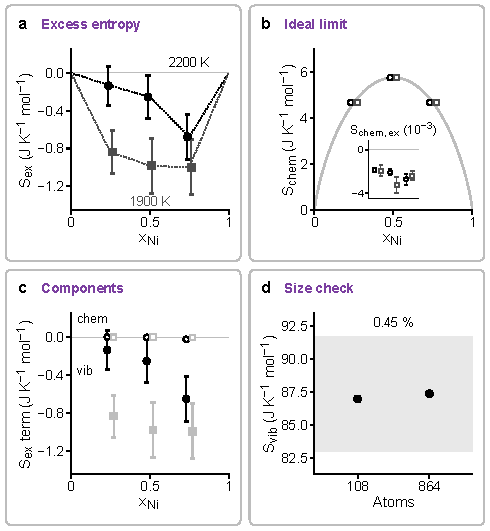
\includegraphics[width=83mm]{fig_crni_entropy_1col}
    \caption{Excess entropy of the Cr--Ni liquid from molecular dynamics, in \unit{\J\per\K\per\mole} of atoms, at \qty{2200}{\K} (circles) and \qty{1900}{\K} (squares), with 108 atoms and \qty{100}{\ps} of production. (a)~Total excess entropy; the error bars do not include the error of the potential. (b)~Ideal-limit check: with the species labels permuted at random, the pair estimator returns the ideal entropy of mixing (grey). (c)~Vibrational (filled) and chemical (open) excess terms. (d)~Cell-size check at Cr$_{50}$Ni$_{50}$ and \qty{2200}{\K}: 108 and 864 atoms differ by 0.45\%, within the $\pm 5\%$ criterion. The pure-Cr reference at \qty{1900}{\K} crystallized after \qty{82}{\ps} and is evaluated over its first \qty{80}{\ps}.}
    \label{fig:entropy}
\end{figure}

The excess entropy of the liquid at each composition and temperature corresponds to the entropy of the mixture minus the entropies of the pure liquids at the same temperature and the ideal entropy of mixing. For Cr--Ni, this quantity is small and negative, ranging between about $-0.1$ and $-1.0$~\unit{\J\per\K\per\mole} (\cref{fig:entropy}a), and it is dominated by the vibrational contribution, with the chemical contribution being two orders of magnitude smaller (\cref{fig:entropy}c). The excess entropies enter the fit as observations, with an uncertainty that combines the statistical error of the simulations with the error of the estimator, and they determine the temperature coefficient of the liquid parameter through the relation $S^{\mathrm{ex}} = -x_{\mathrm{Cr}} x_{\mathrm{Ni}} \sum_k b_k (x_{\mathrm{Cr}} - x_{\mathrm{Ni}})^k$. The use of 108-atom cells is accepted when the vibrational entropy at the equiatomic composition differs by less than 5\% from the value obtained with 864 atoms, a criterion that is met in this case with a difference of 0.45\% (\cref{fig:entropy}d). The excess electronic entropy, on the other hand, is assumed to be zero, since in a metallic liquid this contribution arises only from the change in the density of states at the Fermi level with respect to the pure liquids, and it is expected to be small in comparison with the uncertainty of the vibrational term.

\subsection{Objective and fitting sequence}
\label{sec:methods:objective}
\label{sec:methods:sequence}

We combine the evidence, the one-shot energies, and the entropy of the liquid into a single objective function, and the construction and optimization of this function is the part of the assessment most often left undocumented. In this work, we refine the model with PhaseForge+~\cite{sariturk2025phaseforgeplus}, maximizing the likelihood of ESPEI~\cite{bocklund2019espei} using \emph{analytical gradients of the CALPHAD model fitting error} obtained via the Jansson derivative method~\cite{kunselman2024analytically,kunselman2025analytical}, with pycalphad as the engine for calculating equilibria. Here we note that gradient-based CALPHAD  model optimization is truly enabling, as it reduces the CALPHAD model fit to a multi-dimensional gradient-based optimization problem where all the model parameters can be optimized at once, a radically different approach compared to the standard CALPHAD ad-hoc practice of piecewise model parameter fitting. It is also important to point out that this gradient-based CALPHAD fit~\cite{kunselman2025analytical,kunselman2026hmc} is also orders of magnitude faster than the standard MCMC approach in ESPEI~\cite{bocklund2019espei}.

Since the name of a software environment does not guarantee its contents, the version of ESPEI actually imported during each run is recorded in the run cards. Before the fit, we also compare the analytical gradients term by term with those of ESPEI 0.9.0, at the reference parameters and at a few random points, and with finite differences. Each observation enters the likelihood with the weight implied by its own uncertainty (\cref{sec:methods:orchid}), without multipliers set by hand. Even observations with no reported uncertainty are assigned the uncertainty that the rules of ORCHID would give them, rather than the software default.

Two kinds of observations require special treatment in the objective. Phase boundaries reported with only one end of the tie-line known are split into two: the known phase at the reported composition and, in addition, an equilibrium between this phase and the second phase at a vanishing phase fraction. This corresponds to the zero-phase-fraction condition used in ESPEI, which leaves the partner-phase composition to be determined by the model rather than by an estimate made by the assessor. Excluded phases, in turn, enter the objective through the hinge term of PhaseForge+, which penalizes an excluded phase whenever its Gibbs energy approaches the plane defined by the stable phases at the observed state within a margin $\tau$, set to \qty{100}{\J\per\mole} of atoms by default. Since the most certain tiers correspond to small energy scales, we smooth the onset of this penalty to prevent the optimizer from stalling. As noted earlier (\cref{sec:methods:orchid}), the energy scale of each exclusion is the larger of the certainty tier and the state uncertainty, converted to energy. We obtain the driving-force scale of each zero-phase-fraction record similarly, using the record's uncertainty and its tier as a lower bound.

The fit itself follows a sequence that starts at the liquid and moves down in temperature, in the same order in which experienced CALPHD assessors tend to approach a given system. This order reflects the fact that fewer phases compete at high temperatures, where the liquidus provides a well-defined set of constraints and where one-shot energetics, together with liquid entropy, already restrict the range of acceptable model parameters before the more crowded solid-state region is considered. In the first step, the liquid and the solid phases that melt are therefore fitted to the liquidus, the solidus and the melting invariants, as well as to the excess entropy of the liquid. In the second step, the calorimetric and activity data are added with their own uncertainties; in the last step, the phase-boundary data, the dense assemblages, and the excluded phases are added. Throughout the sequence, a held phase is never fixed. Instead, it remains free and is anchored to its one-shot value through an observation carrying the uncertainty of that value, since fixing a compound at its one-shot energy can leave it stable in regions where it has not been observed, as was the case for CrNi$_2$ in an early version of this assessment. To detect such problems early, the phase diagram is calculated and inspected (by AI agents) after every step, and any step that changes the phase diagram's topology is reported rather than continued.

Since CALPHAD model optimization objectives (i,e., the likelihood) usually have several local optima, each step of the sequence is fitted from multiple starting points, and each start must be polished to convergence before it can be compared to the others. A start is considered to have converged when the norm of the gradient, in the scaling used by the optimizer, falls below a threshold that is stated before the fit ($10^{-3}$ by default), or when it reaches a point at which none of the one-sided directional derivatives can improve the objective---the need for this second condition arises from the fact that the CALPHAD model fitting objective is only piecewise smooth: wherever an observation lies on a phase boundary of the model, the stable assemblage changes at that point, and it is then not possible for the norm of the gradient to become small, even at a true optimum. This same feature also tends to make the fitness landscape quite rugged. For this reason, we follow multistart with basin hopping~\cite{wales1997basinhopping} and dual annealing~\cite{xiang1997dualannealing}, as implemented in SciPy~\cite{virtanen2020scipy}, both starting from the best local result, with a fixed evaluation budget and a random seed set in advance. We record the complete trajectory of each start, including the objective, its individual terms, and the full parameter vector at every evaluation, along with the results; starts without this history are labeled as such, without attempting to reconstruct the missing trajectory by interpolation.

Among the converged starts, the fit carried forward to the next step is chosen by ranking rather than by a threshold on the objective function. Candidate energies are first filtered for plausibility, requiring compound energies to lie within about \qty{10}{\kilo\joule\per\mole} (atom) of the one-shot energies, thermochemical residuals to be on the order of their uncertainty, and pure-element limits to match those of SGTE. In this way, a \emph{fit that achieves the correct topology at the expense of implausible energies cannot be selected}. The plausible candidates are then ranked according to the topology of their phase diagrams, that is, the type of each reaction, the extent of each field, and the absence of spurious phases, with a spurious phase at practical temperatures counted as more serious than one far above the liquidus. Only after this are the remaining candidates ranked according to their quantitative agreement with the data, first in terms of the invariant temperatures and then in terms of the thermochemical residuals of each dataset. Ties between nearly equivalent candidates are resolved by the objective value and never by quantities read from a calculated grid.

\subsection{Physical checks and uncertainty}
\label{sec:methods:checks}
\label{sec:methods:uq}

The ranking described above can only choose among the models produced by the fit. A model with a higher likelihood, however, is not necessarily more physically sound. The general protocol therefore includes a set of checks that are independent of the objective. The \emph{first} of these checks is a gate on the pure elements, for which the phase sequence and melting points must coincide with those of the SGTE descriptions, with ordered end-members equal to their disordered parent. The \emph{second} check concerns the liquid, which must remain convex in composition wherever no liquid miscibility gap has been reported or suspected. The \emph{third} check concerns the possible appearance of a miscibility gap in the solid solution phases. Such a split is not penalized by the objective, since a single-phase observation is satisfied equally well by the two coexisting composition sets, and it can therefore appear in a fit without any cost. For this reason, in the absence of any report of a miscibility gap, and when the mixing energies do not suggest one, a convexity constraint is applied to the phase at its observed single-phase states. The constraint is imposed only above a temperature $T_{\mathrm{allow}}$, the highest temperature at which a metastable gap can be accepted, leaving a concavity that is real but metastable at lower temperatures to the data.

The temperature $T_{\mathrm{allow}}$ is set before the fit, based on two estimates of the critical temperature of a possible miscibility gap. The first estimate corresponds to the incoherent (stress-free) gap. In this case, the regular-solution limit $T_c \approx \Omega/2R$ (with $\Omega$ from the energy of mixing at the equiatomic composition) provides an upper bound, which is then corrected for short-range order and excess vibrational entropy. The second estimate corresponds to the coherent gap, and it is obtained by adding the elastic term of Cahn~\cite{cahn1961spinodal} to the curvature of the Gibbs energy, with elastic constants and lattice parameters calculated with the potential. We report both estimates, along with their uncertainty, derived from the potential error in $\Omega$. The coherent estimate, however, describes the decomposition of a coherent solid solution, not the stable equilibrium represented by the CALPHAD description. A gap that disappears once such corrections have been applied, and that no source reports, supports the use of the convexity constraint. A gap that survives them, on the other hand, remains a real possibility, and for this reason it is left to the data.

Once a model has been chosen, its uncertainty is estimated at low cost from the optima already found during the multistart. For this purpose, the converged starts from the final step are grouped into distinct modes by their parameters, with two starts assigned to different modes when their parameters differ by more than the reproduction tolerances, even if their objectives are nearly equal. This criterion matters because, as described above, the objective is nearly flat in some directions, so two distinct minima can have almost the same posterior value. At each mode, we compute the Hessian of the negative log posterior via central differences of the analytical gradient, then approximate the posterior as a mixture of Laplace approximations~\cite{tierney1986laplace}, with weights that depend on the posterior value at each mode and the determinant of the corresponding Hessian. Parameter vectors drawn from this mixture with a fixed seed are classified on a \qty{5}{\K} grid over the assessment temperature range, according to their topology, invariant temperatures, miscibility gaps, and spurious fields. This classification provides the probability of the accepted topology and its alternatives, along with their binomial errors, and allows the model uncertainty to propagate to any feature of the phase diagram. Markov chain Monte Carlo sampling~\cite{honarmandi2019bayesian,kunselman2026hmc}, which is much more expensive, is not part of the protocol by default and is used only when approved and recorded as a decision.

\subsection{Packaging and reproduction}
\label{sec:methods:package}

The fit, the checks and the estimate of uncertainty described so far all lead to a thermodynamic database, but under the proposed ORCHID-SAGE standard, an assessment is considered complete only when this database is delivered together with the documents that produced it. The database itself carries a header that states how, with which potential, and from which parent files it was generated, while its body remains byte-identical to the file produced by the fit. 

Together with the database, the package contains the specific protocol, the run cards, the evidence bundle, and the assessment dashboard. These documents are assembled into a Workflow Run RO-Crate~\cite{soilandreyes2022rocrate,leo2024wrroc}, in which the specific protocol is the workflow that was actually run and the general protocol is the workflow on which it is based. The run cards, in turn, become actions with their instruments, inputs, outputs, and times, which can be mapped onto the vocabulary of PROV-O~\cite{lebo2013provo} in order to follow the provenance of any result. Inputs that are not part of the crate, such as restricted sources, appear in it only through their hashes and access conditions.

Of these documents, the dashboard is the one intended to make the record accessible to a person. It consists of a single standalone page that is rendered from the evaluation results document, and that can be read without access to a network. For each observed state, the dashboard shows whether the calculated phases correspond to those that were expected, and it also shows the trajectory of the starts in each step of the fit, the evolution of the fit in model space, the residuals of the datasets, the physical checks, the uncertainty, and the decisions taken along the way (\cref{fig:dashboard-objective,fig:dashboard-optimizer,fig:dashboard-parameters,fig:dashboard-projection}). To allow anyone to recompute the projection into model space from the recorded parameter vectors, this projection is deterministic. The parameters are first divided by stated scales and centered on the mean of the retained vectors, then projected onto the two leading eigenvectors of their covariance, with the sign of each eigenvector fixed by its largest component (\cref{fig:dashboard-projection}). Quantities not yet computed are shown as pending, with the reason, and are never filled in with estimates.

Although the dashboard is meant to be read by a person, reproducing a database requires a single command (\texttt{orchid\_reproduce.py}), which needs only the specific protocol and an empty directory. In the first stage, this command copies the code and the assessment evidence into the directory, checks every file against its recorded hash, and verifies that the interpreter matches the recorded environment. In the second stage, it executes the reproduction plan of the specific protocol and compares the new results with the original ones. As discussed in \cref{sec:methods:levels}, the verdict of this comparison is based on the predictions of the two databases, together with byte-for-byte checks of the identity of the data, while differences in the fitted parameters, in the environment, or in the labels of the starts are reported as notes. Steps that cannot be reproduced bitwise, such as relaxations and molecular dynamics simulations performed with GPUs or refits performed with a different processor architecture, are precisely those for which tolerances must be declared. Finally, an independent rerun of the complete specific protocol on a different machine is one of the gates a database must pass before release, and we report this rerun for Cr--Ni in \cref{sec:reproduction}.

\subsection{Machine execution through the Model Context Protocol}
\label{sec:methods:mcp}

The documents described so far can be read by a machine, but a record that a machine can read is not yet, necessarily, a record that a machine can carry out. In order to close this gap, the protocols, run cards, evidence bundles, validator, reproduction tools, and dashboards of ORCHID-SAGE are exposed through a server based on the Model Context Protocol~\cite{mcp}, alongside the existing ORCHID server for the data, so that an AI agent can use them as tools, resources, and prompts. In reproduction mode, an agent without prior context can list available protocols, read the steps of a specific protocol with exact commands, inputs, outputs, and tolerances, and verify that the inputs match the recorded hashes. The agent can then obtain a reproduction plan, run it one step at a time, and compare the outputs with those of the original assessment. Since some steps, such as the fits, take hours, they start in the background, and the agent follows their progress through a separate status call so no step depends on a single call remaining open. For a judgment step, on the other hand, the server returns the decision recorded in the specific protocol, together with its source, so that the agent applies the decision that was actually made instead of making one of its own.

In addition to reproducing existing assessments, the same server can start a new assessment for a system that has not yet been assessed. In this case, the server instantiates a draft of the specific protocol from the general protocol in a fresh directory and opens a request for each decision the general protocol leaves to a person, such as the choice of phases, the temperature range, and the source of the unary descriptions. It then gathers the evidence from the local ORCHID data, with certainty tiers and excluded phases at the observed states, and works through the steps of the general protocol in order. It runs computable steps, produces a job specification for steps that require a GPU, and pauses judgment steps until a person answers the corresponding request with a name and a reason the server cannot supply on its own. Because every step writes a run card, an assessment started this way is reproducible from its first step. However, in its present form, this mode has two limitations: fitting a new system still requires a person to adapt the reference code, which is then recorded as a change of tool, and there is not yet a dashboard for an assessment started this way.

In both modes, people remain free to change a protocol, provided that they document the change within the schema. A change to a specific protocol is recorded as a departure from the step of the general protocol it modifies, along with a decision stating who made the change, when, why, and on what evidence. Such a change produces a new version of the specific protocol, which must be validated before it is accepted; the steps affected by the change, as well as those that depend on them, are then marked as stale and rerun, while their earlier run cards are kept. A change to the general protocol, in turn, produces a new version of this protocol and never an edit of a released one, and an assessment moves to the new version only through a recorded decision. In this work, for example, correcting an error in the evidence bundle construction and a race condition between parallel workers led to new versions of both the evidence and the specific Cr--Ni protocol, while all earlier versions remained unchanged.

Since an agent acts on the record through these tools, the server has also been designed to prevent the agent from damaging the record it is reading. All runs take place in fresh directories that the server creates and marks, and these directories cannot be located inside the repository, the active campaigns, or the data copies. Each command is checked before it is executed, and a command that writes outside its directory, deletes files, or connects to another host is refused. In addition, the system runs a single step per call, after explicit confirmation that must be repeated for long steps such as fits. The server does not run steps that require a GPU, and the person must enable remote machines. Finally, none of the server tools can delete a file or access the network, and restricted sources are hashed to verify their presence but are never read out or copied.

\subsection{AI assistance and human decisions}
\label{sec:methods:ai}

The server safeguards are a particular case of a more general division of work between AI agents and (expert) humans, intended to leave the agents with steps that can be checked against the record and to reserve to people the decisions that cannot. In the assessment of Cr--Ni, AI agents (Claude Opus 5.5, Anthropic) working under the general protocol carried out most of the steps, from the search of the literature and the extraction and verification of the evidence to the one-shot calculations, the optimization of the model and the assembly of the specific protocol, the run cards and the dashboard. In contrast, the present author made the decisions that the protocol reserves to expert humans, including selecting phases, accepting new records, and adopting a new rule whenever a result revealed that one was missing. The protocol's decision log documents each of these decisions, including the date, the person responsible, the justification, and the source on which the decision is based whenever one exists. Decisions agents make on their own appear in the same log, where they are identified as such. Records extracted for this work from a single reading, finally, remain flagged until a second reader has verified them against the original source.

In this sense, the decision log also documents how the evidence has shaped the method. Several rules in the general protocol were introduced in response to specific results from this assessment and earlier ones. Examples include the requirement to specify excluded phases at all observed states, the rule that held parameters are anchored rather than fixed, the treatment of transforming structures through the midpoint of their relaxation interval and the lower bound on the energy scale of each exclusion. Each of these rules is now part of the standard, and the result that motivated it is recorded together with it. Thus, a protocol under ORCHID-SAGE constitutes a version of the method, one that evolves as new evidence requires and in which the assessor's judgment remains free, provided that the exercise of this judgment is documented.
